\chapter{Output Feedback}
\label{output_feedback}

Chapter \ref{state_feedback} introduced the concept of reachability. It was shown that it is possible to find 
a state feedback law that gives the desired closed loop eigenvalues provided that the system
is reachable.  Furthermore, we saw how to design controllers using
the system state, $x(t)$, as feedback to out controller. 

However, desigining state feedback controllers preassumes that all the states are measured. For many situations, it
is highly unrealistic to assume that all the states are measured. 

In this section we proceed somehow in a similar vein we can use the output $y(t)$ to modify the dynamics of the system through the use of observers. Furthermore, we will introduce the concept of observability
and show that if a system is observable, it is possible to recover the state
from measurements of the inputs and outputs to the system. We then show how to
design a controller with feedback from the observer state. 




\section{Observability}
\label{observability}

For many situations, it is highly unrealistic to assume that all the states are measured. In this section we
investigate how the state can be estimated by using a mathematical model and a
few measurements. It will be shown that computation of the states can be carried
out by a dynamical system called an \textbf{observer}, see also figure \ref{observer_block_diagram}.


\begin{framed}
\theoremstyle{definition}
\begin{definition}{\textbf{Observability}}
A linear system is \textbf{observable}  if for any $T>0$ it is possible to determine the state of the system $x(T)$ through measurements of $y(t)$ and $u(t)$ on the interval $[0,T]$  $x(T) = x_f$.
\end{definition}
\end{framed}


\begin{framed}
\theoremstyle{remark}
\begin{remark}{\textbf{Nonlinear Systems}}

The definition above holds for nonlinear systems as well, and the results discussed here have extensions to the nonlinear case.
\end{remark}
\end{framed}


Consider again the system

\begin{equation}
\frac{dx}{dt} = Ax + Bu ~~ y = Cx + Du
\end{equation}


where $x\in R^n$ is the state, $u\in R^{p}$ is the input and $y\in R^q$ the measured output.

We wish to estimate the state of the system from its inputs and outputs, as illustrated
in Figure \ref{observer_block_diagram}. In some situations we will assume that there is only one measured
signal, i.e., that the signal $y$ is a scalar and that $C$ is a (row) vector. This signal may
be corrupted by noise $n$, although we shall start by considering the noise-free case.
We write $\hat{x}$ for the state estimate given by the observer.

\begin{figure}[!htb]
\begin{center}
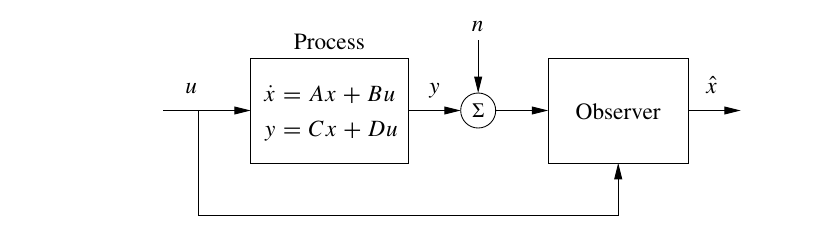
\includegraphics[scale=0.380]{img/output_feedback/observer_block_diagram.jpeg}
\end{center}
\caption{Block diagram for an observer. The observer uses the process measurement $y$
(possibly corrupted by noise $n$) and the input $u$ to estimate the current state of the process,
denoted $\hat{x}$.}
\label{observer_block_diagram}
\end{figure}


The problem of observability is one that has many important applications, even
outside feedback systems. If a system is observable, then there are no hidden dynamics inside it; we can understand everything that is going on through observation (over time) of the inputs and outputs. As we shall see, the problem of observability is of significant practical interest because it will determine if a set of sensors is
sufficient for controlling a system. Sensors combined with a mathematical model
can also be viewed as a virtual sensor that gives information about variables that
are not measured directly. The process of reconciling signals from many sensors
with mathematical models is also called sensor fusion.



\section{Testing for Observability}
\label{test_observability}

When discussing reachability in the last chapter, we neglected the output and focused on the state. Similarly, it is convenient here to initially neglect the input and
focus on the autonomous system



\begin{framed}
\theoremstyle{remark}
\begin{remark}{\textbf{Autonomous System}}

\end{remark}
\end{framed}

\begin{equation}
\frac{dx}{dt} = Ax ~~ y = Cx
\end{equation}

The objective is to understand when it is possible to determine the state from observations of the output. From

\begin{equation}
y = Cx
\end{equation}

we see that the output itself gives us the projection of the state $x$ on vectors that are rows of the matrix $C$. The 
observability problem can  immediately be solved if the matrix $C$ is invertible. If the matrix is not invertible we can take the derivatives and obtain

 
\begin{equation}
\frac{dy}{dt} = C\frac{dx}{dt} = CAx
\end{equation}

From the derivative of the output we thus get the projection of the state on vectors that are rows of the matrix $CA$. Proceeding in this way, we get

\begin{equation}
\begin{bmatrix}
 y \\
 y^{(1)} \\
 \vdots \\
 y^{(n-1)} 
\end{bmatrix} = 
\begin{bmatrix}
 C \\
 CA \\
 \vdots \\
 CA^{n-1} 
\end{bmatrix}x
\end{equation}

We thus find that the state can  be  determined if the observability matrix
 
\begin{equation}
W_o= 
\begin{bmatrix}
 C \\
 CA \\
 \vdots \\
 CA^{n-1} 
\end{bmatrix}
\end{equation}

has $n$ independent rows.  It turns out  that  we  need  not consider any derivatives higher
than $n-1$ (this is an application of the Cayley-Hamilton theorem)
 
\begin{framed}
\theoremstyle{remark}
\begin{remark}{\textbf{System with inputs}}

The calculation can easily be extended to systems with inputs. The state is then
given by a linear combination of inputs and outputs and their higher derivatives.
The observability criterion is unchanged. 
\end{remark}
\end{framed}


\begin{framed}
\theoremstyle{theorem}
\begin{theorem}{\textbf{Observability rank condition}}

A linear system of the form  
\begin{equation}
\frac{dx}{dt} = Ax + Bu, ~~ y = Cx + Du \nonumber
\end{equation}

is observable if and only if the observability matrix $W_o$ is full rank.
\end{theorem}
\end{framed}

\section{Observable Canonical Form}
\label{observability_canonical_form}

As in the case of reachability, certain canonical forms will be useful in studying ob-
servability. A linear single-input, single-output state space system is in observable
canonical form if its dynamics are given by


\begin{framed}
\theoremstyle{remark}
\begin{remark}{\textbf{Observable Canonical Form for Nonlinear Systems}}

The definition can be extended to systems with many inputs; the only difference is
that the vector multiplying u is replaced by a matrix.
\end{remark}
\end{framed}


The characteristic polynomial for a system in observable canonical form is

\begin{equation}
\lambda(s) = s^n +\alpha_1s^{n-1} + \ldots + \alpha_{n-1}s + \alpha_n
\end{equation}

In order to check the observability property of a systme more formally, we can compute the observability matrix for
a system in observable canonical form. This is given by

\begin{equation}
W_o= 
\begin{bmatrix}
 1 & 0 & 0 & \ldots &  0\\
 -\alpha_1 & 1 & 0 & \ldots &  0 \\
 -\alpha_{1}^{2} - \alpha_1 \alpha_2 & - \alpha_1 & 1 &  \ldots &  0 \\
 \vdots & \vdots & \vdots & \ddots & \vdots \\
* & * & * & \ldots & 1
\end{bmatrix} 
\end{equation}


where * represents  an entry  whose exact  value  is  not important.
What is important here is the rows of this matrix are linearly independent (since it is lower triangular), and hence Wo is full rank. Hence, it is invertible. 

As in the case of reachability (see section \ref{reachable_canonical_form}), it  turns  out  that  if a  system  is  observable then there
always exists a transformation $T$ that converts the system into observable canonical
form. This is useful for proofs since it lets us assume that a system is in observable
canonical form without any loss of generality. The observable canonical form may
be poorly conditioned numerically.
 

\section{State Estimation}
State feedback control design, as explained in t chapter \ref{state_feedback} requires that we have access to the complete state vector. 
However, measuring the complete state vector is not always feasible (for example a sensor may not be available at all) and it may also be expensive.
In this section we will introduce the idea of state estimation as a way to get access to the state variables. 


\begin{framed}
\theoremstyle{remark}
\begin{remark}{\textbf{Soft Sensors}}


The concept of using software instead of sensors to access the quantity we are 
interested in, is referred to as soft sensors in the automotive industry.
\end{remark}
\end{framed}

Recall that the idea of state feedback control was to modify the eigenvalues of the system under consideration by using the input

\begin{equation}
u = -Kx + K_r r  
\end{equation}

However, it can be seen that this requires the state vector $x$. The idea of state estimation is to design something called an observer that tries to provide an 
estimate say $\hat{x}$ of the state vector $x$. The observer is fed with the same input as the real plant. The goal of the observer is to provide somehow a replica of the true state vector.
Thus, we would like to have the error $\tilde{x}$ between the two quantities to be zero. Namely,


\begin{equation}
\tilde{x} = x - \hat{x} = 0 
\end{equation}
 
In this section, we want to construct a dynamical system of the form

\begin{equation}
\frac{d \hat{x}}{dt} = F\hat{x} + Gu + Hy  
\end{equation}

where $u$ and $y$ are the input and output of the original system and $\hat{x} \in R^n$ is an estimate of $x$ with the property

\begin{equation}
\hat{x}(t) \rightarrow x(t), ~~ \text{as} ~~ t \rightarrow \infty  
\end{equation}

Let's consider again the system

\begin{equation}
\frac{dx}{dt} = Ax + Bu ~~ y = Cx + Du
\label{sys}
\end{equation}

assume further that $D$ is zero. Assuming that the input $u$ is known, then an estimate of the state $x$ is given by

\begin{equation}
\frac{d\hat{x}}{dt} = A\hat{x} + Bu
\label{observer_one} 
\end{equation}  

We would like to know the properties of this estimate; how far is from the exact state? The estimation error is \cite{Astrom} 

\begin{equation}
\tilde{x} = x - \hat{x} 
\end{equation} 

substituting into equation \ref{observer_one} we find that


\begin{equation}
\frac{d\tilde{x}}{dt} = A\tilde{x}  
\end{equation}  

We already know that the behavior of this system depends on the eigenvalues of $A$. Concretely, if matrix $A$ has all its eigenvalues in the left half-plane, the error $\tilde{x}$ will go to zero,
and hence equation \ref{observer_one} is a dynamical system whose output converges to the state
of the system \ref{sys}.


The observer given by equation \ref{observer_one} uses only the process input $u$; the measured
signal does not appear in the equation. We must also require that the system be stable,
and essentially our estimator converges because the state of both the observer and
the estimator are going zero. This is not very useful in a control design context since
we want to have our estimate converge quickly to a nonzero state so that we can
make use of it in our controller. We will therefore attempt to modify the observer
so that the output is used and its convergence properties can be designed to be fast
relative to the system’s dynamics. This version will also work for unstable systems.

Let's now consider the following observer

\begin{equation}
\frac{d \hat{x}}{dt} = A\hat{x} + Bu + L(y- C \hat{x})
\label{observer_two}   
\end{equation}

The term $L(y- C \hat{x})$ provides feedback and hence the observer in \ref{observer_two} can be seen as a generalization of the observer in \ref{observer_one}. The supplied feedback is proportional to the difference between the observed output and the output predicted by the observer. Substituting the expression for the error $\tilde{x}$ we arraive at

 \begin{equation}
\frac{d\tilde{x}}{dt} = (A-LC)\tilde{x} 
\label{observer_two}   
\end{equation} 

If the matrix $L$ can be chosen in such a way that the matrix $A-LC$ has eigenvalues with negative real parts, the error $\tilde{x}$ will go to zero. The convergence rate is determined by an appropriate selection of the eigenvalues.
 

\begin{framed}
\theoremstyle{remark}
\begin{remark}{\textbf{Observer design and state feedback duality}}


Notice the similarity between the problems of finding a state feedback and
finding the observer. State feedback design by eigenvalue assignment is equivalent
to finding a matrix $K$ so that $A-BK$ has given eigenvalues. Designing an observer
with prescribed eigenvalues is equivalent to finding a matrix $L$ so that $A-LC$ has
given eigenvalues. Since the eigenvalues of a matrix and its transpose are the same
we can establish the following equivalences:

\begin{equation}
A \leftrightarrow A^T, ~~ B \leftrightarrow C^T, ~~ K \leftrightarrow L^T, ~~ W_r \leftrightarrow W_{o}^{T}
\end{equation}

The observer design problem is the dual of the state feedback design problem. 
\end{remark}
\end{framed}



\begin{framed}
\theoremstyle{theorem}
\begin{theorem}{\textbf{Observer design by eigenvalue assignment}}


Consider the system

\begin{equation}
\frac{dx}{dt} = Ax + Bu, ~~ y =Cx   \nonumber
\end{equation} 

with one input and one output. Let the characteristic polynomial related to matrix A be

\begin{equation}
\lambda(s) = s^n + \alpha_1 s^{n-1} + \ldots + \alpha_{n-1}s + \alpha_n \nonumber
\end{equation}

If the systme is observable, then the dynamical system

\begin{equation}
\frac{d \hat{x}}{dt} = A\hat{x} + Bu + L(y- C \hat{x})  \nonumber
\end{equation}


is an observer for the system with $L$ chosen as 

\begin{equation}
L = W_{o}^{-1}\tilde{W}_o
\begin{bmatrix}
 p_1 - \alpha_1 \\
 p_2 - \alpha_2 \\
 \vdots  \\
 p_n - \alpha_n
\end{bmatrix} \nonumber
\end{equation}

The matrices $W_{o}$ and $\tilde{W}_{o}$ are given by

The resulting observer error $\tilde{x}$ is governed by a differential equation that has the following characteristic polynomial

\begin{equation}
p(s) = s^n +  p-1 s^{n-1} + \ldots + p_n  \nonumber
\end{equation}
\end{theorem}
\end{framed}

The dynamical system (7.10) is called an observer for (the states of) the system (7.9) because it will generate an approximation of the states of the system from its inputs and outputs. This form of an observer is a much more useful form than the one given by pure differentiation in equation (7.3).


\section{Questions}

\textbf{Question 1}

What is the main reason for using an estimator in feedback control?

\begin{itemize}
\item A) There are process disturbances in the model 
\item B) We are measuring the wrong quantities 
\item C) It is too expensive or impractical to measure each state variable correct 
\end{itemize} 

\textbf{Answer}  

Option C is the correct answer.

